\chapter{Bearbeitung der Übungsaufgaben}

\section{Differenzenquotient}

Um die erste Ableitung $\frac{\mathrm{d}f}{\mathrm{d}x}(x)$ einer hinreichend glatten skalaren Funktion $f: \mathbb{R} \rightarrow \mathbb{R}$ an der Stelle $x$ numerisch zu approximieren kann man den rechtsseitigen (\ref{rechtsseitig}) und den zentralen (\ref{zentral}) Differenzenquotienten 

\begin{align}
	&\frac{\mathrm{d}f}{\mathrm{d}x}(x) = \frac{f(x+h)-f(x)}{h} + \mathcal{O}(h) \label{rechtsseitig}
	\\	
	&\frac{\mathrm{d}f}{\mathrm{d}x}(x) = \frac{f(x+h)-f(x-h)}{2h} + \mathcal{O}(h^{2})
	\label{zentral}
\end{align}

nutzen wobei die Schrittweite $h \neq 0$ sehr klein zu wählen ist. Mit Hilfe der Taylorentwicklung inklusive Restgliedabschätzung wird im Folgenden die Konvergenzordnung der obigen Differenzenquotienten ermittelt. An der Stelle $f(x+h)$ lautet das allgemeine Taylorpolynom zweiten Grades 

\begin{equation*}
	T_2f(x+h)= f(x) +f'(x)h +\frac{f''(\xi)}{2!}h^2
\end{equation*}

mit der Fehlerabschätzung $f''(\xi)$ an einer unbekannten Stelle $\xi$ mit $ x <\xi <(x+h)$. Diese Gleichung umgestellt nach der gesuchten ersten Ableitung $f'(x)$ ergibt 

\begin{equation}
	f'(x) = \frac{f(x+h)-f(x)}{h}-\frac{f''(\xi)}{2}h
	\label{mitFehler}
\end{equation}

und mit der oberen Abschätzung für den Fehler folgt 

\begin{equation}
	f'(x) = \frac{f(x+h)-f(x)}{h}+\mathcal{O}(h).
	\label{ohneFehler}
\end{equation}

Hier wird jetzt ersichtlich, dass die Korrektur des rechtsseitigen Differenzenquotienten linear abhängig zur Schrittweite $h$ ist und somit eine Konvergenz 1. Ordnung hat. Konvergenz 1. Ordnung heißt in diesem Fall, dass durch eine Halbierung der Schrittweite $h$ auch die Fehlerabweichung halbiert wird.\\
Aus den Taylorpolynomen dritten Grades an den Stellen $f(x+h)$, siehe (\ref{(x+h)}) und $f(x-h)$, siehe (\ref{(x-h)})

\begin{align}
	&T_3f(x+h)= f(x) + f'(x)h +\frac{f''(x)}{2!}h^2 + \frac{f'''(\xi_r)}{3!}h^3
	\label{(x+h)}
	\\
	&T_3f(x-h)= f(x) - f'(x)h +\frac{f''(x)}{2!}h^2 - \frac{f'''(\xi_l)}{3!}h^3
	\label{(x-h)}
\end{align}

mit den Unbekannten $\xi_r$ und $\xi_l$, $(x-h) < \xi_l < x < \xi_r < (x+h)$, folgt nach den selben Schritten wie zuvor bei (\ref{mitFehler}) und (\ref{ohneFehler}) 

\begin{equation*}
	f'(x) = \frac{f(x+h)-f(x-h)}{2h} + \mathcal{O}(h^2).
\end{equation*}

Der zentrale Differenzenquotient hat also eine Konvergenz 2. Ordnung, da die Korrektur quadratisch von der Schrittweite $h$ abhängt. Konvergenz zweiter Ordnung bedeutet, dass bei einer Halbierung der Schrittweite nur noch ein Viertel des Fehlers gemacht wird.\\
Um einen Differenzenquotient 4.Ordnung für die erste Ableitung zu konstruieren reichen nicht mehr nur zwei Punkte zum Approximieren aus, stattdessen benötigt man jetzt 4 verschiedene Punkte $f(x-h)$, $f(x-\frac{h}{2})$, $f(x+\frac{h}{2})$ und $f(x+h)$ und kombiniert zwei zentrale Differenzenquotienten. Mit der selben Vorgehensweise wie zuvor lässt sich dann nachweisen, dass der Differenzenquotient

\begin{equation*}
	\frac{\mathrm{d}f}{\mathrm{d}x}(x) = \frac{f(x+h)-f(x-h)+2f(x+\frac{h}{2})-2f(x-\frac{h}{2})}{4h}
\end{equation*}

von Konvergenz 4. Ordnung ist.\\

Um die Unterschiede der verschiedenen Differenzenquotienten graphisch darzustellen, bietet es sich an diese für verschieden große Schrittweiten $h$ sowie für verschiedene Funktionen zu testen. Getestet wird mit elf verschiedenen Schrittweiten $h \in [10^{-10},1]$ und den Funktion $f(x) = \exp(x+1)$ (siehe Abbildung \ref{fig:eFunktion}) an der Stelle $x=1$, $g(x) = \cos(x)$ (siehe Abbildung \ref{fig:cosinus}) an der Stelle $ x = \frac{\pi}{2}$ und der in Abbildung \ref{fig:Polynom} dargestellte absolute Fehler der Funktion

\begin{equation}
	h(x)=
		 \begin{cases}
			6x^2+ 4 & x>1\\
			4x^3+6 & x\leq 1
		\end{cases}
	\label{polynom}
\end{equation}

an der Stelle $x=1$. Die im Anhang zu findende Octave-Routine \texttt{Aufgabe4\_1} ermittelt den absoluten Fehler zwischen der tatsächlichen, analytisch bestimmten Ableitung der Funktionen und der numerischen Approximation mit den drei Differenzenquotienten. Zur Darstellung wird ein doppelt logarithmischer Plot verwendet, dadurch können sowohl die kleineren als auch die größeren Werte in einem Schaubild dargestellt werden.\\
Auffällig ist, dass bei jeder der drei Testfunktionen die kleinste Schrittweite nicht die beste Annäherung liefert, sondern es einen Tiefpunkt bei etwa $h=10^{-5}$ bzw. $h=10^{-8}$ gibt. Das bedeutet, dass ab diesem Punkt durch weiteres verkleinern der Schrittweite keine höhere Genauigkeit der Approximation erzielt werden kann. Außerdem erkennt man dass bei allen drei Verfahren die Größe der Fehler weitgehend ähnlich ist, mit Ausnahme der Approximation der Exponential-Funktion(\ref{fig:eFunktion}), bei der der rechtsseitige Differenzenquotient einen deutlich größeren Fehler erzeugt. 
Für Schrittweiten größer als das Optimale $h$ zeigen alle Graphen lineares Verhalten. Für den Wert der Steigung ist die Konvergenzordnung ausschlaggebend, wie im Folgenden noch gezeigt wird. 
\begin{figure}[thbp]
	\centering
	\begin{subfigure}[tpbh]{0.68\textwidth}
		\centering
		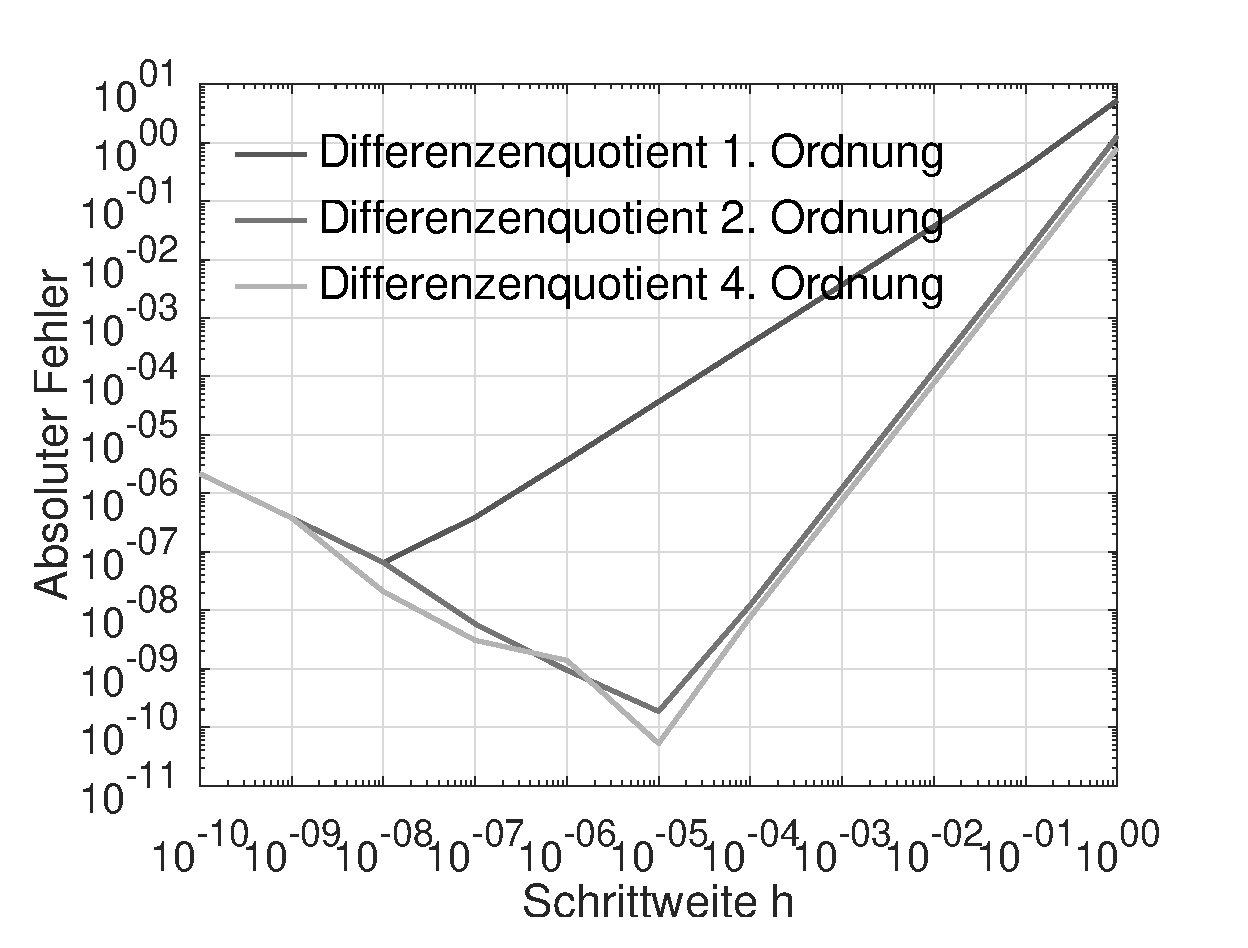
\includegraphics[width=\textwidth]{data/eFunktion}
		\caption{Fehler bei der Approximation von $f(x) = \exp(x+1)$ an der Stelle $x=1$}
		\label{fig:eFunktion}
	\end{subfigure}
	\begin{subfigure}[tpbh]{0.68\textwidth}
		\centering
		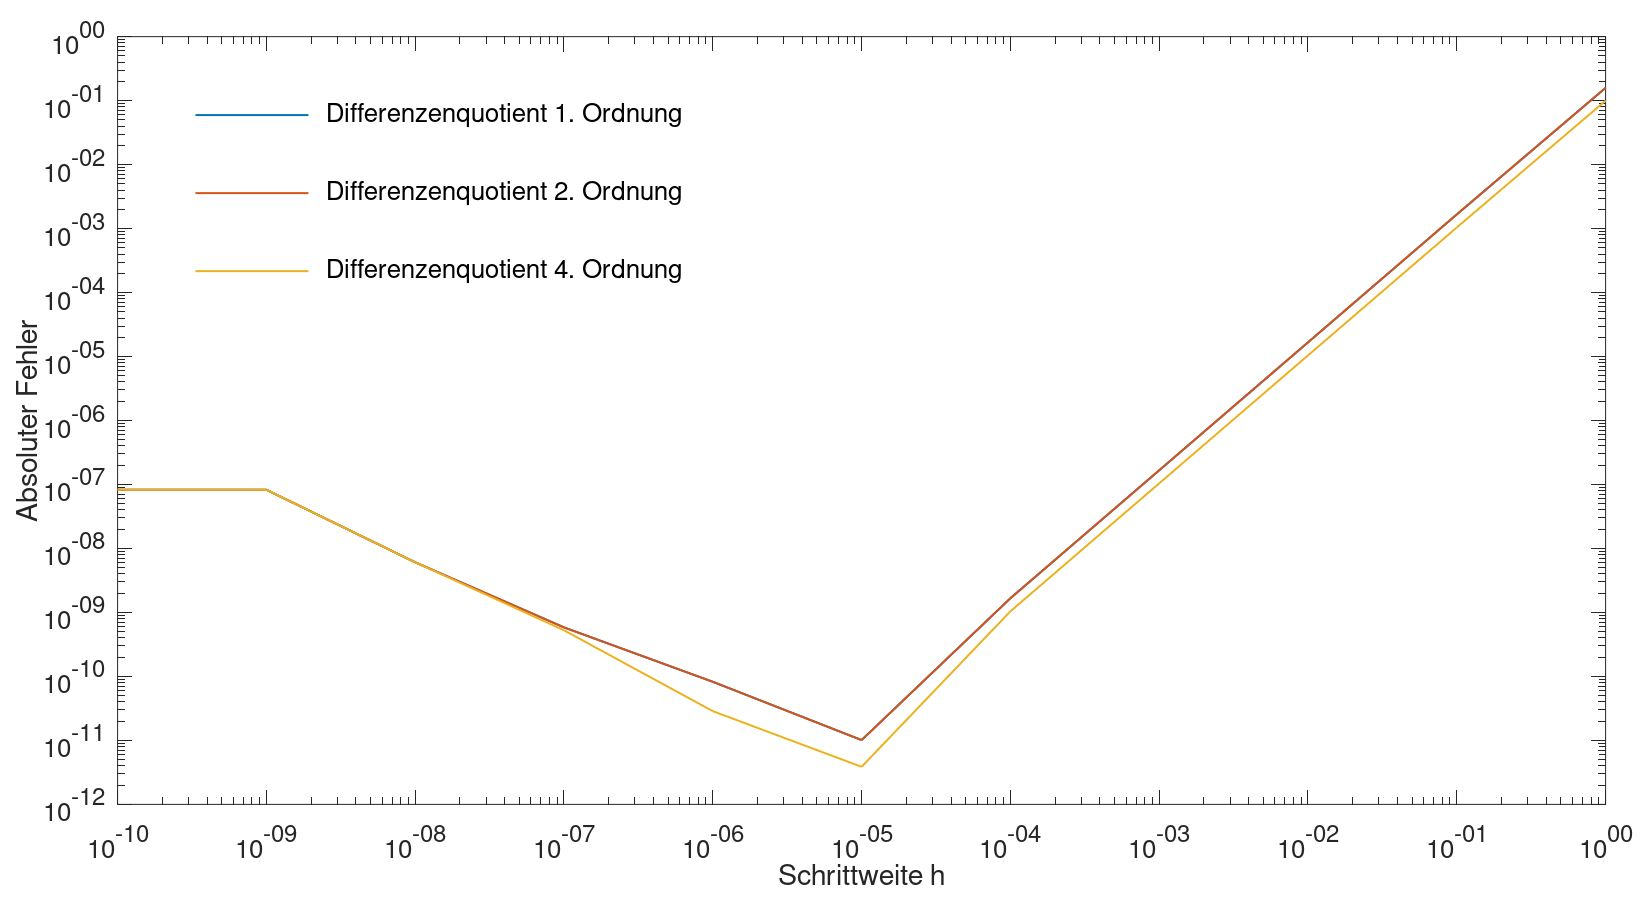
\includegraphics[width=\textwidth]{data/sinus}
		\caption{Fehler bei der Approximation von $g(x) = \cos(x)$ an der Stelle $x=\frac{\pi}{2}$}
		\label{fig:cosinus}
	\end{subfigure}
	\begin{subfigure}[tpbh]{0.68\textwidth}
		\centering
		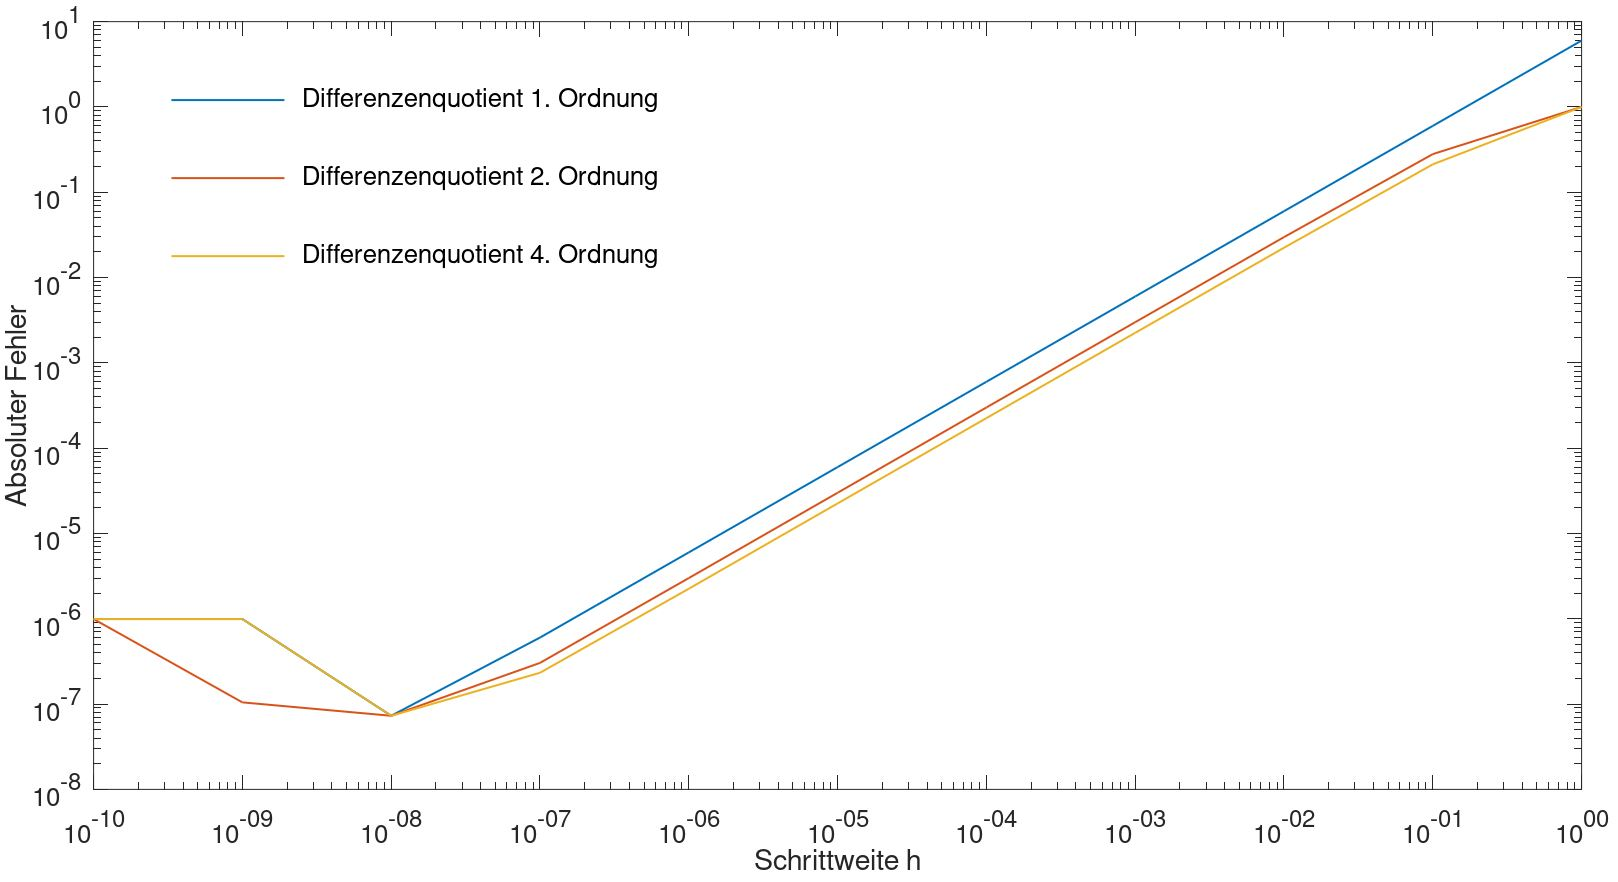
\includegraphics[width=\textwidth]{data/abschnittsFkt}
		\caption{Fehler bei der Approximation von (\ref{polynom}) an der Stelle $x=1$ }
		\label{fig:Polynom}
	\end{subfigure}
	\caption{Fehler der numerischen Approximationen der ersten Ableitung im doppelt logarithmischen Koordinatensystem}
	\label{fig:fehlerPlots}
\end{figure}



Um in einem doppelt logarithmischem Koordinatensystem die Steigung einer Geraden zu berechnen (siehe Abbildung \ref{steigung}), reicht es nicht wie bei einem linearen Koordinatensystem die Werte $\Delta x$ und $\Delta y$ des allgemeinen Steigungsdreiecks durch die Differenz der auf den Achsen angegebenen Werte zu ermitteln.\\
Stattdessen wird auf die Werte, die man an den jeweiligen Stellen auf den Achsen ablesen kann, der Logarithmus zur selben Basis angewandt, der zur Erzeugung der logarithmischen Skala verwendet wurde. In diesem Beispiel zur Basis $10$. Der Quotient zur Ermittlung der Steigung lautet dann 

\begin{equation*}
	\frac{\Delta y}{\Delta x} = \frac{\log(C (10^{\Delta r +r})^p)-\log(C (10^r)^p)}{\log(10^{\Delta r +r}) - \log(10^r)}
\end{equation*} 

und unter Anwendung der Logarithmus Regeln $\log(u\cdot v) = \log u + \log v$ und $\log (10^w) = w$ folgt

\begin{equation*}
	\frac{\Delta y}{\Delta x} = \frac{(p(\Delta r +r)-pr)}{r+\Delta r -r}
	=p.
\end{equation*}

Die Steigung der Fehlerabschätzung $\epsilon (h)$ ist somit genau gleich mit der Ordnung $p$ des jeweiligen numerischen Verfahrens zur Approximation.

\begin{figure}[htpb]
	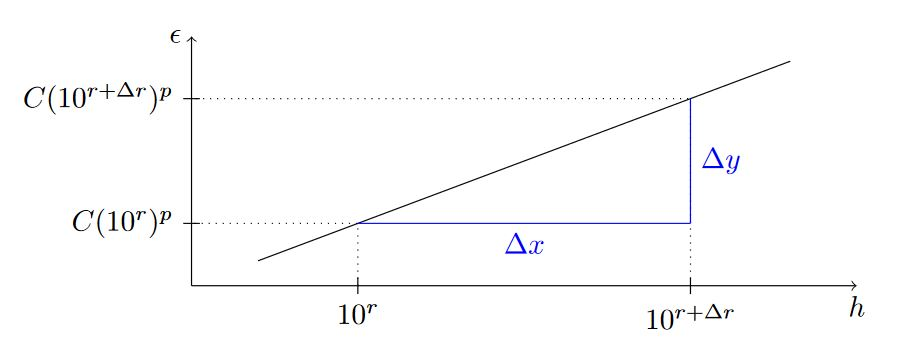
\includegraphics[width=\textwidth]{data/SteigungLogPlot}
	\caption{Allgemeines Steigungsdreieck in einem doppelt Logarithmischen Koordinatensystem}
	\label{steigung}
\end{figure}

Hat das logarithmische Koordinatensystem nicht die Basis 10, sondern eine beliebige andere, ist die Steigung für $\epsilon (h)$ weiterhin durch die Ordnung $p$ gegeben. Zur Berechnung des allgemeinen Steigungsdreiecks wird, wie bereits beschrieben, der Logarithmus zur selben beliebigen Basis auf alle Werte angewendet, somit ist die Basis des Logarithmus unerheblich für die Steigung.





